\documentclass{projetofinal-dcc}
%%%%%%%%%%%%%%%%%%%%%%%%%%%%%%%%%%%%%%%%%%%%%%%%%%%%%%%%%%%%
% P A C O T E S
%%%%%%%%%%%%%%%%%%%%%%%%%%%%%%%%%%%%%%%%%%%%%%%%%%%%%%%%%%%%

\usepackage{listings}
\usepackage{xcolor}
\usepackage{caption}
\usepackage{array}

%%%%%%%%%%%%%%%%%%%%%%%%%%%%%%%%%%%%%%%%%%%%%%%%%%%%%%%%%%%%
% C O N F I G U R A Ç Õ E S  D O S  P A C O T E S
%%%%%%%%%%%%%%%%%%%%%%%%%%%%%%%%%%%%%%%%%%%%%%%%%%%%%%%%%%%%

\definecolor{mGreen}{rgb}{0,0.6,0}
\definecolor{mGray}{rgb}{0.5,0.5,0.5}
\definecolor{mPurple}{rgb}{0.58,0,0.82}
\definecolor{backgroundColour}{rgb}{0.98,0.98,0.97}

\lstdefinestyle{CStyle}{
    backgroundcolor=\color{backgroundColour},   
    commentstyle=\color{mGreen},
    keywordstyle=\color{magenta},
    numberstyle=\color{mGray},
    stringstyle=\color{mPurple},
    breakatwhitespace=false,         
    breaklines=true,                 
    captionpos=b,                    
    keepspaces=true,                 
    numbers=left,                    
    numbersep=5pt,                  
    showspaces=false,                
    showstringspaces=false,
    showtabs=false,                  
    tabsize=2,
    language=C
}

%%%%%%%%%%%%%%%%%%%%%%%%%%%%%%%%%%%%%%%%%%%%%%%%%%%%%%%%%%%%
%I N I C I O  D O  D O C U M E N T O
%%%%%%%%%%%%%%%%%%%%%%%%%%%%%%%%%%%%%%%%%%%%%%%%%%%%%%%%%%%%
\begin{document}

% título da tese é obrigatório
\title{Utilizando Mesh Shaders para Extração Procedural de Isosuperfícies}

% autor é obrigatório; máximo de 3 autores
\author{Vinicius de Assis Sento Sé}{Primeiramente gostaria de agradecer ao meu pai Roberto Ruy Sento Sé Júnior e a minha mãe Janaína Alves de Assis por todo o carinho, educação e amor que me foi dado durante toda minha vida. Gostaria de agradecer ao meu irmão Willian de Assis Sento Sé por ter sido a maior fonte de inspiração e orgulho que eu poderia ter. Sou extremamente grato por toda a motivação vinda de minha madrasta Jaciara da Silva Guilhermino e de minha avó Eva Alves de Assis. Agradecimentos especiais dedicados à minha namorada Vanessa da Costa Nascimento por todo apoio e paciência que demonstrou durante esse período tão importante de minha vida.

Por fim, gostaria de agradecer ao meu orientador Bruno Dembogurski por ter me auxiliado durante este estudo e a todos os meus amigos que me acompanharam durante esta longa jornada. }
%\author{Nome completo aluno 2}{Primeiramente gostaria de agradecer ao meu pai Roberto Ruy Sento Sé Júnior e a minha mãe Janaína Alves de Assis por todo o carinho, educação e amor que me foi dado durante toda minha vida. Gostaria de agradecer ao meu irmão Willian de Assis Sento Sé por ter sido a maior fonte de inspiração e orgulho que eu poderia ter. Sou extremamente grato por toda a motivação vinda de minha madrasta Jaciara da Silva Guilhermino e de minha avó Eva Alves de Assis. Agradecimentos especiais dedicados à minha namorada Vanessa da Costa Nascimento por todo apoio e paciência que demonstrou durante esse período tão importante de minha vida.

Por fim, gostaria de agradecer ao meu orientador Bruno Dembogurski por ter me auxiliado durante este estudo e a todos os meus amigos que me acompanharam durante esta longa jornada. }
%\author{Nome completo aluno 3}{Primeiramente gostaria de agradecer ao meu pai Roberto Ruy Sento Sé Júnior e a minha mãe Janaína Alves de Assis por todo o carinho, educação e amor que me foi dado durante toda minha vida. Gostaria de agradecer ao meu irmão Willian de Assis Sento Sé por ter sido a maior fonte de inspiração e orgulho que eu poderia ter. Sou extremamente grato por toda a motivação vinda de minha madrasta Jaciara da Silva Guilhermino e de minha avó Eva Alves de Assis. Agradecimentos especiais dedicados à minha namorada Vanessa da Costa Nascimento por todo apoio e paciência que demonstrou durante esse período tão importante de minha vida.

Por fim, gostaria de agradecer ao meu orientador Bruno Dembogurski por ter me auxiliado durante este estudo e a todos os meus amigos que me acompanharam durante esta longa jornada. }

% orientador é obrigatório
\advisor[Prof.]{Bruno José Dembogurski,~D.Sc.}{}
% \advisor[Prof.]{Nome completo,~D.Sc.}{}{a} % orientadora

% co-orientador é opcional
%\coadvisor[Prof.]{Nome do co-orientador,~M.Sc.}{}
%\coadvisor[Prof.]{Nome do co-orientador,~M.Sc.}{}{a} % co-orientadora

% máximo de 3 integrantes da banca (orientador e co-orientador já são adicionados automaticamente)
\banca[Prof.]{Marcelo Panaro de Moraes Zamith,~D.Sc.}{DCC~-~UFRRJ}
\banca[Prof.]{Filipe Braida do Carmo,~D.Sc.}{DCC~-~UFRRJ}
%\banca[Prof.]{Nome do participante banca 3,~Ph.D.}{DCC~-~UFRRJ}

\location{Nova Iguaçu}{RJ}{Brasil}

% mês e ano de defesa
\date{Agosto}{2022}
\maketitle

\startdocument
%%%%%%%%%%%%%%%%%%%%%%%%%%%%%%%%%%%%%%%%%%%%%%%%%%%%%%%%%%%%
%A G R A D E C I M E N T O S
%%%%%%%%%%%%%%%%%%%%%%%%%%%%%%%%%%%%%%%%%%%%%%%%%%%%%%%%%%%% 
\makethankspage

%%%%%%%%%%%%%%%%%%%%%%%%%%%%%%%%%%%%%%%%%%%%%%%%%%%%%%%%%%%%
%R E S U M O
%%%%%%%%%%%%%%%%%%%%%%%%%%%%%%%%%%%%%%%%%%%%%%%%%%%%%%%%%%%%
\begin{abstract}{
  Em 2018, a NVIDIA anunciou um novo módulo programável para suas GPUs capaz de aprimorar o fluxo de renderização atual denominado de mesh shaders. Com o intuito de explorar suas novas funcionalidades, estudamos seu uso um contexto de geração de geometria procedural. Para isto, desenvolvemos uma ferramenta com capacidade de compilar e executar mesh shaders. Com o auxilio dessa ferramenta, pudemos observar a performance e o uso dos recursos durante a execução do algoritmo de marching cubes. Por fim, comparamos os resultados obtidos com a implementação do mesmo algoritmo em compute shaders.

Palavras chave: mesh shaders, geometria procedural, marching cubes.
}
\end{abstract}

%%%%%%%%%%%%%%%%%%%%%%%%%%%%%%%%%%%%%%%%%%%%%%%%%%%%%%%%%%%%
%A B S T R A C T
%%%%%%%%%%%%%%%%%%%%%%%%%%%%%%%%%%%%%%%%%%%%%%%%%%%%%%%%%%%%
\begin{englishabstract}{
  In 2018, NVIDIA announced a new programable module for theirs GPUs capable of improve the current rendering flow. In order to explore its new features, we studied their use in the context of procedural geometry generation. For that, we developed a tool able to compile and execute mesh shaders. With that, we could observe the performance and resource usage during de marching cubes algorithm execution. Finally, we compare the results with the compute shader implementation.
}
\end{englishabstract}

%%%%%%%%%%%%%%%%%%%%%%%%%%%%%%%%%%%%%%%%%%%%%%%%%%%%%%%%%%%%
%L I S T A S
%%%%%%%%%%%%%%%%%%%%%%%%%%%%%%%%%%%%%%%%%%%%%%%%%%%%%%%%%%%%
% Figuras
\makefigurespage

% Tabelas
\maketablespage

% Algoritmos
%\makelistingspage

% Abreviaturas (devem estar em ordem alfabética)
%\makeabrevpage{\input{elementos-pretextuais/abreviaturas}}

% Símbolos (devem estar em ordem alfabética)
%\makesymbolspage{\input{elementos-pretextuais/simbolos}}

% Sumário 
\maketocpage

%%%%%%%%%%%%%%%%%%%%%%%%%%%%%%%%%%%%%%%%%%%%%%%%%%%%%%%%%%%%
%C O N T E Ú D O
%%%%%%%%%%%%%%%%%%%%%%%%%%%%%%%%%%%%%%%%%%%%%%%%%%%%%%%%%%%%
\startcontent
\chapter{Introdução}\label{chp:LABEL_INTRODUCAO}


Em tempos modernos, a manipulação de grandes quantidades de dados se tornou uma necessidade inquestionável para diversas áreas da sociedade. No contexto da computação gráfica, isso pode ser retratado pela alta fidelidade visual desejável em aplicações em tempo real.

Com o poder de processamento gráfico moderno, já é possível gerar imagens computacionais que se assemelham da realidade. Em fevereiro de 2017, uma emissora de televisão aberta confundiu durante uma reportagem em rede nacional um video de jogabilidade do jogo de videogame \textit{Forza Motorsport 6}, lançado em 2015, com um video de testes para motorista do presidente dos Estados Unidos.

Ainda que novas tecnologias tenham permitido que esse tipo de aplicação alcançasse uma qualidade gráfica satisfatória, dado sua linearidade na preparação dos dados de entrada, o processo atual responsável pela geração das imagens virtuais em tempo real não consegue se manter eficiente conforme a quantidade de dados cresce para magnitudes mais altas. Este problema afeta diretamente aplicações mais intensas, como é visto em experiencias em realidade virtual ou ferramentas CAD (computed aided design).

Dado esse contexto, desenvolvedores e artistas trabalharam em novos meios de aprimorar a qualidade gráfica sem incrementar a malha das geometrias \textit{renderizadas}. Contudo, isso provocou um significativo aumento na complexidade do do fluxo, que então se tornou inflexível e imprevisível. \cite{TECR_MESH_SHADERS_DIRECTX_12}

Por volta de 2015, pesquisadores começavam a esboçar a abstração de \textit{meshlets}, uma nova modelagem de dados capaz de otimizar o processo de renderização. A ideia de meshlets consiste em pré-processar a malha, aprimorando a reutilização de vértices, eliminando os índices duplicados e removendo lotes de geometria que não serão visíveis na imagem final. Embora esta fosse uma técnica eficaz para cenas estáticas, a rígida estrutura de entrada da esteira vigente restringia seus ganhos de performance em ambientes dinâmicos, como é visto em cenas com muito movimento ou em geração de geometria procedural.

Visando mitigar as restrições da esteira de renderização atual, a fabricante de componentes de aceleração gráfica \textit{NVIDIA} introduziu em 2018 a sua arquitetura nomeada \textit{Turing} \cite{TECR_TURING_ARCHITETURE} o conceito de \textit{mesh shaders}: um novo módulo programável capaz de remodelar a esteira de renderização por completa. Além de simplificar o fluxo graças ao seu modelo de programação CPM (compute programing model), mesh shaders possibilitam a flexibilização da estrutura dos dados de entrada, permitindo assim um uso mais eficiente dos recursos da GPU.

\section{Objetivo}

Com o intuito de explorar as novas capacidades providas da esteira de renderização baseada em mesh shaders, foi desenvolvido para esse estudo uma ferramenta capaz de visualizar e comparar a execução do algoritmo de geração de geometria procedural \cite{REF_BOOK_PROCEDURAL_MODELING} denominado de \textit{marching cubes}. \cite{REF_ART_MARCHING_CUBES}. Este que pode se beneficiar das novas funcionalidades do novo módulo de programação por ser computacionalmente custoso porém completamente paralelizável.

\section{Organização do Documento}

O Capitulo \ref{chp:LABEL_FUND_TEORICA} introduz os conceitos técnicos necessários para o entendimento do estudo. O Capítulo \ref{chp:LABEL_CASOS_DE_ESTUDOS} comentaremos sobre o algoritmo de marching cubes, implementado para este trabalho utilizando mesh shaders. No Capítulo \ref{chp:LABEL_EXPERIMENTOS}, apresentamos a ferramenta desenvolvida e os experimentos executados. 
Por fim, no Capítulo \ref{chp:LABEL_CONCLUSAO}, concluiremos a nossa pesquisa com os resultados obtidos e trabalhos futuros.
\chapter{Fundamentação Técnica}\label{chp:LABEL_CASOS_DE_ESTUDOS}

Neste capítulo abortaremos o algoritmo de geração de \textit{isosupercícies} procedurais conhecido como Marching Cubes, escolhido para realizar a comparação entre os pipelines por se beneficiar das novas funcionalidades trazidas pelos mesh shader.

\section{O Algoritmo Marching Cubes}\label{sec:LABEL_CASOS_DE_ESTUDOS_SEC_A}

\begin{figure}
\centering
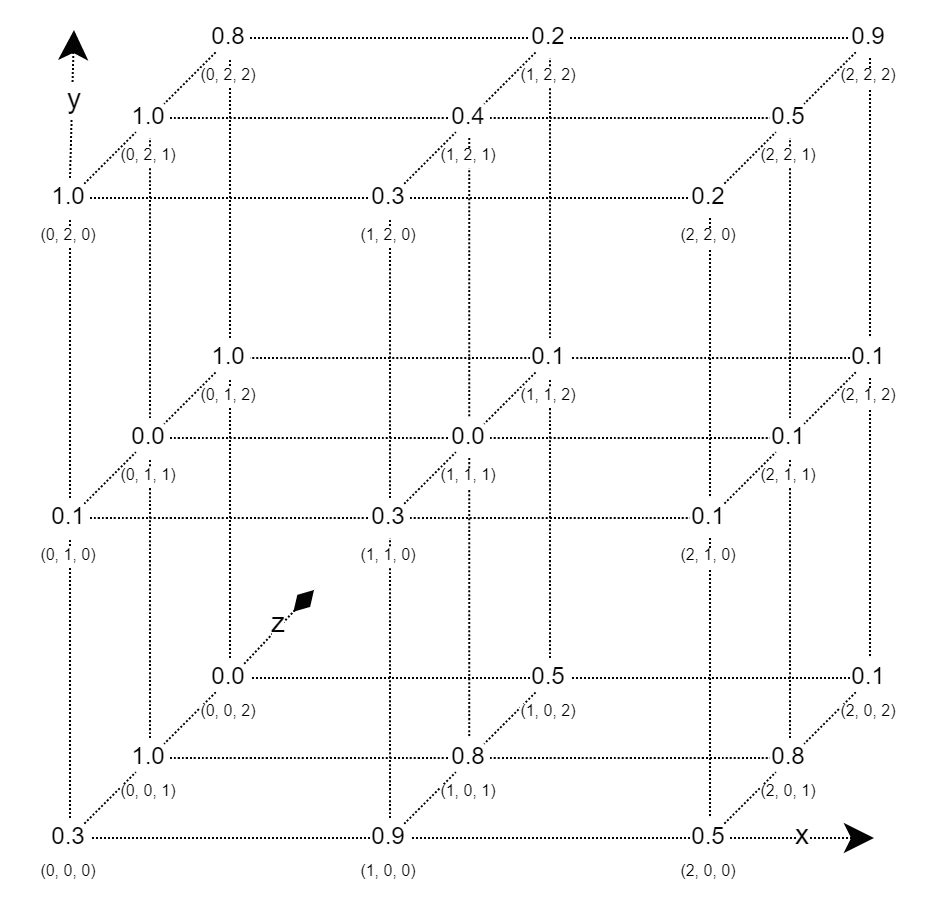
\includegraphics[width=0.6\textwidth]{imagens/MarchingCubes-NuvemDensidade.png}
\caption{Representação da densidade atribuída às coordenadas espaço}
\label{fig:LABEL_FIG_NUVEM_DENSIDADE}
\end{figure}

Proposto em 1987 para a visualização tridimensional dos resultados de exames de tomografias computadorizadas, Marching cubes \cite{REF_ART_MARCHING_CUBES} é um algoritmo capaz de construir superfícies de alta resolução utilizando uma abordagem de dividir para conquistar. Com o avanço na capacidade de processamento do hardware atual, o algoritmo obteve diversas outras usabilidades na área da computação gráfica. Como por exemplo no remapeamento na topologia de malhas complexas \cite{REF_ART_MARCHING_CUBES_REMESH} ou na geração dinâmica de terrenos proceduras em jogos eletrônicos \cite{REF_ART_MARCHING_CUBES_TERRAIN_GENERATION}.


Dado a representação volumétrica da superfície, denominada \textit{nuvem de pontos}, ilustrada pela Figura \ref{fig:LABEL_FIG_NUVEM_DENSIDADE}, o algoritmo percorre as sub sessões do espaço de interesse auxiliado por uma tabela de pesquisa chamada de \textit{tabela de triangularização}. A tabela de triangularização dita quais vértices serão conectados para formar os triângulos que irão compor a malha. Quanto menor for o tamanho das sub sessões, maior é a quantidade de triângulos construídos e, consequentemente, maior é o nível de detalhe da geometria final. 

Embora utilize apenas operações lógicas simples, marching cubes pode ser um algoritmo computacionalmente custoso quando requer um maior nível de detalhe da superfície. Visto que cada sub sessão pode ser percorrida individualmente, sua execução é altamente paralelizável. 

\section{Nuvem de pontos}\label{sec:LABEL_CASOS_DE_ESTUDOS_SEC_B}

A nuvem de pontos consiste em uma matriz cúbica de pontos. Um ponto é um vetor que possui duas informações: posição e densidade. Enquanto a primeira representa sua posição no espaço, a segunda armazena um valor entre 0 e 1 que é utilizado para determinar se aquele ponto está dentro ou fora da superfície. O \textit{nível da superfície} é um número constante $l$ que indica o valor mínimo de densidade necessária para um ponto estar dentro da superfície. Dado um ponto arbitrário p, diz-se que p está dentro da superfície se e somente se $densidade(p) \geq l$. Caso contrário, o ponto está fora da superfície.


Dado uma região no espaço tridimensional, a construção da nuvem de pontos se dá ao distribuir pontos em intervalos regulares dentro desta região. Visando manter as proporções da malha pelas 3 dimensões em 1:1:1, deve-se atribuir a mesma quantidade de pontos igualmente entre elas. Com os pontos distribuídos, aplica-se para cada ponto, uma função $f$ tal que $f(x, y, z) => d$, onde $x$, $y$ e $z$ são as coordenadas do ponto no espaço e $d$ é a densidade atribuída a aquele ponto. A disposição de densidades no espaço junto do nível da superfície ditam a silhueta da geometria que será construída.

\section{Geração dos Triângulos}\label{sec:LABEL_CASOS_DE_ESTUDOS_SEC_C}

\begin{figure}
\centering
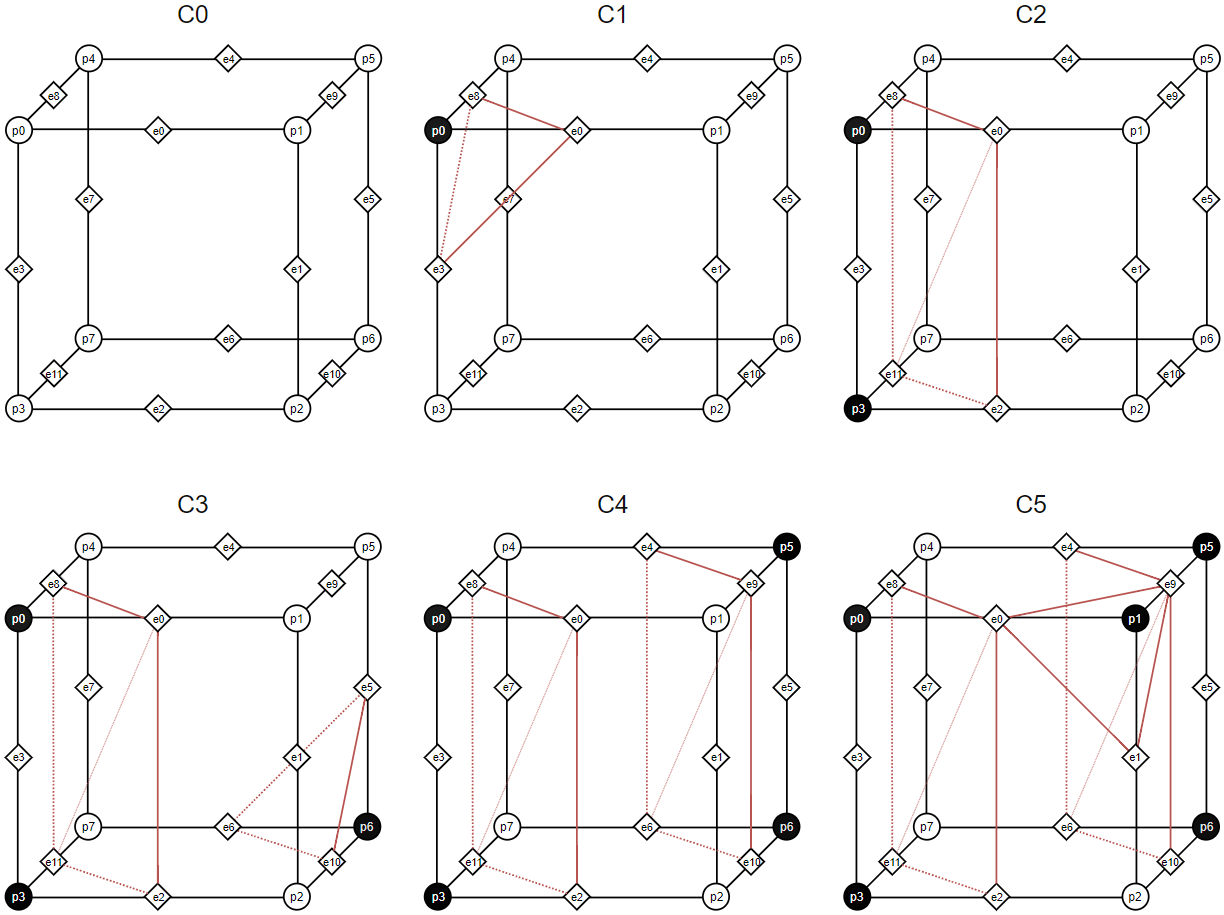
\includegraphics[width=0.9\textwidth]{imagens/MC-ConfiguracoesCubo.png}
\caption{Representação das distintas configurações de cubo}
\label{fig:LABEL_FIG_CONFIGURACOES_CUBO}
\end{figure}

Após a construção da nuvem de pontos, os pontos presentes nesta são agrupados 8 a 8, de forma que cada ponto represente a vértice de um cubo com arestas de tamanho máximo $k$, onde $k$ é a distancia entre dois pontos vizinhos arbitrários na nuvem de pontos. Para cada cubo gerado, verifica-se a configuração dos pontos que o representa. O objetivo do algoritmo é construir triângulos que separem os pontos que estão fora da superfície dos que estão dentro.

Visto o exemplo ilustrado na figura \ref{fig:LABEL_FIG_CONFIGURACOES_CUBO}, a configuração $C0$ não apresenta nenhum ponto dentro da superfície, logo não necessita da criação de triângulos. Já em $C1$, o ponto $p1$ é indicado como dentro da superfície, então um triangulo é gerado conectando as arestas $e0$, $e3$ e $e8$. Em $C2$, além de $p1$, $p3$ também está fora da superfície, então são construídos dois triângulos: o triangulo $e0$, $e8$ e $e11$ e o triangulo $e0$, $e2$ e $e11$. Considerando que cada ponto contém apenas duas possibilidades de estados: dentro ou fora da superfície e que um cubo é composto por 8 pontos, existem um total de $2^8 = 256$ possibilidades distintas de triangularização. Entretanto, apenas 14 dessas são configurações únicas, sendo o restante apenas variações de rotação destas. Para auxiliar a tarefa de construção dos triângulos, o algoritmo de marching cubes utiliza de uma tabela de pesquisa. Cada linha desta tabela representa uma configuração distinta de cubo e indica quais arestas devem ser conectadas para formar um triangulo.

Afim de se construir geometrias mais \textit{aredondadas}, incrementando seu nível de detalhe, a posição das vértices dos triângulos é interpolada de acordo com a densidade dos pontos que a representam. Dado dois pontos adjacentes $p0$ e $p1$, suas respectivas posições no espaço $\overrightarrow{P0}$ e $\overrightarrow{P1}$ e o nível da superfície $l$, a posição $\overrightarrow{P}$ do vértice do triangulo construído sob a aresta que os intercepta se da pela seguinte formula:


\begin{equation}
    \overrightarrow{P} = \overrightarrow{P0} + \frac{l - densidade(p0)}{densidade(p1) - densidade(p0)} * (\overrightarrow{P0} - \overrightarrow{P1})
\end{equation}

A Figura \ref{fig:LABEL_FIG_INTERPOLACAO} ilustra a diferença visual obtida através dessa melhoria.

\begin{figure}
\centering
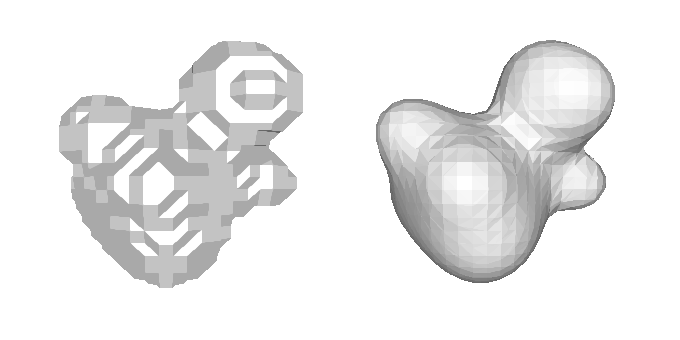
\includegraphics[width=0.6\textwidth]{imagens/PontoMedioXInterpolado.png}
\caption{Malha interpolada pelo ponto médio dos vértices (à esquerda) e sua representação interpolada pela média de densidade dos pontos adjacentes (à direita) }
\label{fig:LABEL_FIG_INTERPOLACAO}
\end{figure}

Conforme ilustrado na figura \ref{fig:LABEL_FIG_EXECUCAO_ALGORITIMO}, o algoritmo então marcha por todos os possíveis cubos presentes no espaço adicionando os vértices criados a uma lista de vértices e índices que serão repassados para o pipeline de rasterização posteriormente.

\begin{figure}
\centering
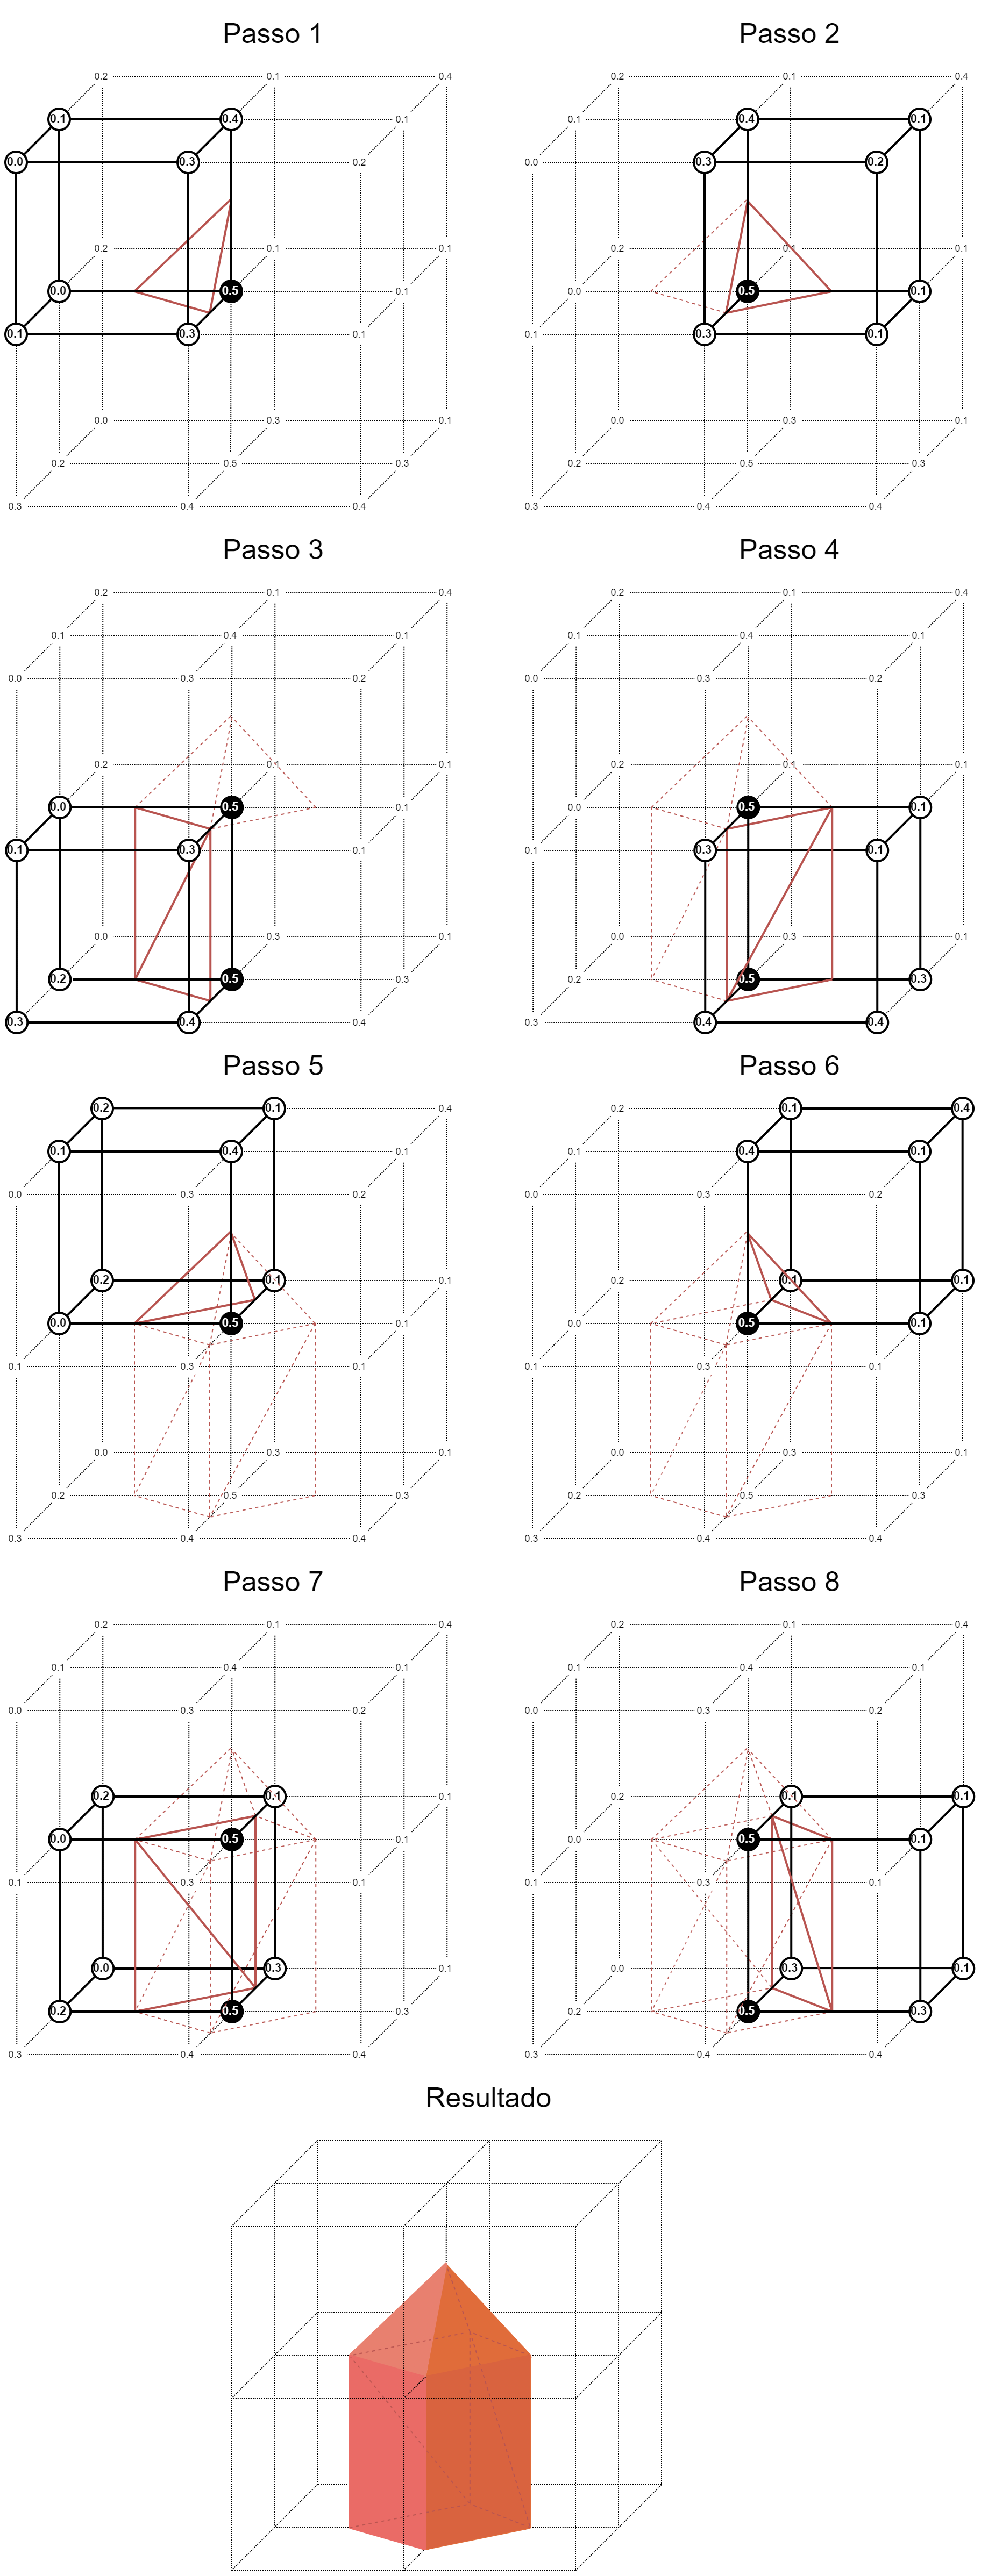
\includegraphics[width=0.6\textwidth]{imagens/MarchingCubes-Execucao.png}
\caption{Passo a passo da execução do algorítimo de marching cubes}
\label{fig:LABEL_FIG_EXECUCAO_ALGORITIMO}
\end{figure}

\section{Complexidade}\label{sec:LABEL_CASOS_DE_ESTUDOS_SEC_D}

Cado a natureza cúbica da nuvem de pontos, a quantidade de interações cresce na terceira potencia. Uma nuvem contendo 2 pontos em cada dimensão possuí um total de 8 pontos. Neste caso, apenas um cubo pode ser formado, então o algorítimo executará apenas uma interação. Caso incrementemos um 1 ponto em cada dimensão esta nuvem possuirá então 27 pontos no total, podendo agora formar 8 cubos distintos. Logo, 8 interações são executadas. Dado uma nuvem cúbica com $n$ pontos distribuídos uniformemente nas 3 dimensões, temos que a quantidade de pontos presentes nesta se por $n ^ 3$. Já a quantidade de cubos formados é definida por $\lfloor\frac{n ^ 3}{8}\rfloor$. Com isto, observamos que a complexidade do algoritmo de marching cubes é da ordem de $\mathcal{O}(n^3)$

Considerando uma região de interesse no espaço de $10m^3$, caso deseja-se construir uma isosuperfície com precisão de $1m$, deve-se distribuir $10$ pontos distanciados igualitariamente entre as 3 dimensões dentro deste intervalo. Dependendo da distribuição de densidade dos pontos, conforme exemplificado em \ref{sec:LABEL_CASOS_DE_ESTUDOS_SEC_B}, múltiplas combinações de triangularizações podem ser geradas. Embora não seja trivial de visualizar, a combinação de triangularização mais complexa contém um total de 5 triângulos. Tomando esse como pior dos casos, podemos estimar que a quantidade máxima triângulos com 10 pontos é de $10^3*5 = 5000$ triângulos.

\begin{figure}
\centering
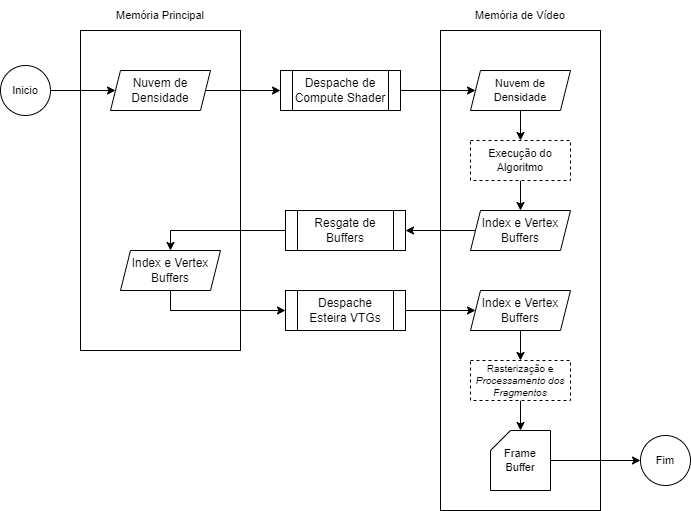
\includegraphics[width=0.9\textwidth]{imagens/FluxoDados-RendIndireta.drawio.png}
\caption{Fluxograma dos dados em renderização indireta}
\label{fig:LABEL_FIG_REND_INDIRETA}
\end{figure}

\section{Implementações}\label{sec:LABEL_FLUXO_DOS_DADOS}

O algoritmo de marching cubes pode ser implementado de forma eficiente em duas distintas configurações: renderização indireta através de compute shaders ou renderização direta com mesh shaders.

Conforme comentado na Sessão \ref{sec:LABEL_RENDERIZACAO_INDIRETA}, os dados processados com compute shaders devem ser renderizados de forma indireta. A Figura \ref{fig:LABEL_FIG_REND_INDIRETA} ilustra a sequencia de etapas necessárias para a implementação do marching cubes. O fluxo inicia-se com a pré-montagem da nuvem de densidades da geometria a ser renderizada. Após o despache do compute shader, a nuvem de dados é armazenada em um SSBO. Após a execução do algoritmo, os index e vertex buffers gerados são armazenados em um segundo SSBO que pode ser resgatado através de uma chamada a API gráfica. Como compute shaders não se comunicam com o fluxo de renderização, os dados computados por ele devem retornar a memória principal antes de serem tramitados para um programa de renderização VGTs.

Já no segundo fluxo, ilustrado pela figura \ref{fig:LABEL_FIG_REND_DIRETA}, temos uma sequencia mais otimizada. Após a execução do algoritmo de marching cubes, os index e vertex buffers são repassados diretamente para a rasterização, onde são fragmentados sem a necessidade de retornar a memória principal.

\begin{figure}
\centering
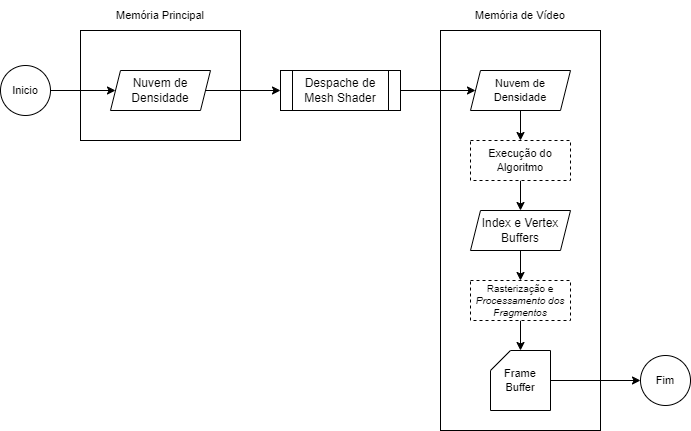
\includegraphics[width=1\textwidth]{imagens/FluxoDados-RendDireta.drawio.png}
\caption{Fluxograma dos dados em renderização direta}
\label{fig:LABEL_FIG_REND_DIRETA}
\end{figure}
\chapter{Fundamentação Teórica}\label{chp:LABEL_FUND_TEORICA}

Tendo em vista que o foco principal desse estudo é a comparação entre a esteira de renderização vigente e sua versão aprimorada utilizando mesh shaders em aplicações dinâmicas, Este capitulo abordará os conceitos básicos por trás da esteira de renderização atual e os novos módulos maleáveis de programação em contexto gráfico.

\section{Esteira de renderização}\label{sec:LABEL_CHP_1_SEC_PIPELINE_RENDERIZACAO}

O termo \textit{renderizar} remete-se à ideia de sintetizar mídias processadas através do computador. Em computação gráfica, este termo é utilizado para se referir à construção de imagens digitais. A esteira, ou, \textit{pipeline} de renderização, consiste em uma sequencia de etapas fixas e programáveis cujo o propósito é desenhar um ou mais objetos em uma cena.

A técnica mais utilizada para a renderização de imagens em aplicações em tempo real é a \textit{rasterização}. A rasterização consiste na transformação de uma imagem vetorial, montada através de um conjunto de vetores denominados de \textit{vértices}, em um conjunto de \textit{rasters} (ou pixels\footnote{menor ponto de uma imagem bidimensional convencional}). Um vértice é uma estrutura de dados que representa o menor ponto no espaço. Além de suas coordenadas, vértices podem armazenar outras informações como cor, vetor normal, coordenada de textura, etc. O produto da rasterização é escrito no \textit{frame buffer}. O frame buffer é uma região de memória que armazena as informações necessárias para a exibição dos dados computados em um dispositivo de saída de vídeo.

Durante a renderização de uma única imagem, normalmente, centenas de milhares de vértices são rasterizados. Dado que aplicações em tempo real normalmente requerem que diversas imagens sejam exibidas em frações de segundo para se ter a ilusão de movimento e interatividade, a esteira de renderização é majoritariamente executada no hardware otimizado e dedicado à esta tarefa: a GPU (graphics processing units). Por conta da grande diversidade de fabricantes e modelos de GPUs, a interface entre o programador e o hardware é facilitada através de APIs (application program interface)\footnote{Interface de abstração entre linguagens de baixo e alto nível} gráficas como DirectX, Vulkan ou OpenGL. Cada API gráfica possui suas particularidades em funcionalidades e nomenclaturas. Para este estudo, por ser uma ferramenta de código aberto com uma ampla comunidade fornecendo documentações de usabilidade e soluções de problemas, a API escolhida foi o OpenGL. Contudo, os conceitos abordados nesse trabalho podem ser aplicados para as demais APIs.

A programação do pipeline é feita através dos \textit{shaders}. Um shader consiste em uma sequencia de instruções que serão realizadas no hardware de aceleração de vídeo. Atualmente, a esteira de renderização em OpenGL possui 5 principais tipos de shaders: vertex shader, TCS (tessellation control shader), TES (tesselation evaluation shader) \cite{WIKI_OPENGL_TESSELATION}, geometry shader e fragment shader. Durante o decorrer desse trabalho, iremos nos referir a esta esteira como esteira de renderização \textit{VTGs}.

A esteira VGTs necessita de dois dados de entrada: \textit{vertex buffers} e \textit{index buffers}. O vertex buffer consiste em um conjunto de vértices que formarão a geometria a ser renderizada. O index buffer é a estrutura que representa quais vértices devem ser conectados a fim de formar uma \textit{geometria primitiva}. Geometrias primitivas são a base para a construção da superfície do objeto a ser renderizado. Uma geometria primitiva pode ser um ponto, uma reta ou um triangulo. O fluxo inicia-se com o processamento dos vértices pelo vertex shader seguido pelas etapas amplificação de malha (TCS, TES e geometry shaders). Logo após, ocorre a fase de rasterização. Os rasters gerados são processados pelo fragment shader e, por fim, são armazenados no \textit{frame buffer}. Conforme ilustrado na Figura \ref{fig:LABEL_FIG_PIPELINE_ATUAL}.

Shaders podem referenciar locais de memórias compartilhadas chamadas de \textit{uniforms}. Uniforms são variáveis de escopo global implicitamente constantes. Essas variáveis são utilizadas como parametrização da esteira de renderização. Embora os uniforms possam armazenar diferentes estruturas de dados, existem certas restrições em seu uso. A quantidade máxima de componentes uniforms ativos por invocação de shader é limitada pelo estágio da esteira. Isso pode ser um problema quando há a necessidade de utilizar maiores estruturas de dados, como vetores e matrizes de pontos flutuantes.


\begin{figure}
\centering
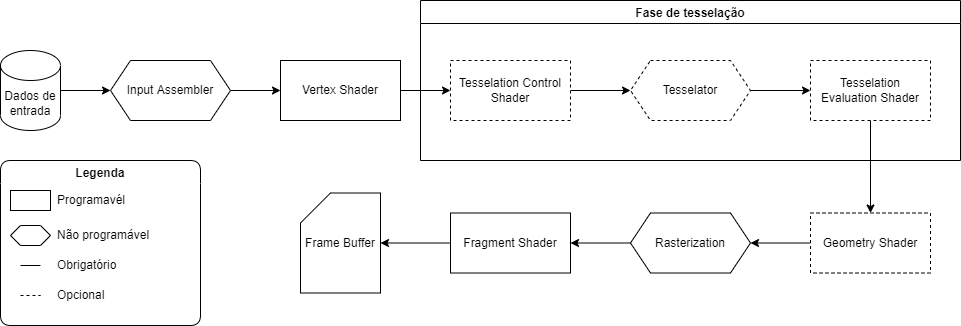
\includegraphics[width=1\textwidth]{imagens/PipelineRenderizacaoOpenGL.png}
\caption{Pipeline de Renderização Atual em OpenGL (Simplificado)}
\label{fig:LABEL_FIG_PIPELINE_ATUAL}
\end{figure}

\section{Compute Shaders}\label{sec:LABEL_CHP_1_SEC_C}

O \textit{compute shader} é um tipo especifico de shader que permite o processamento de grandes quantidades de dados arbitrários distribuídos entre diferentes grupos de trabalhos (\textit{workgroups}). Um workgroup é um conjunto de threads\footnote{Fluxo de execução independente de um programa} que compartilham uma memória de rápido acesso, conforme ilustrado na Figura \ref{fig:LABEL_FIG_WORKGROUPS}. Compute shaders melhor exploram as capacidades do hardware moderno ao flexibilizar a forma em que os dados são processados. O modelo de programação via workgroups permitem que informações transitem entre as unidades de processamento das GPUs sem que haja a necessidade da invocação de outros shaders, possibilitando a execução de algoritmos mais complexos. 

O paradigma computacional dos compute shaders se assemelha ao bibliotecas como OpenCL e CUDA. Entretanto, apesar de compute shaders não conter todas as funcionalidades, seu uso é vantajoso em aplicações em OpenGL pelos seguintes motivos:

\begin{itemize}
  \item Compute shaders são escritos em GLSL, similar à outros shaders escritos para OpenGL;
  \item A validação, compilação e montagem de computer shaders são realizadas da mesma forma que outros shaders em OpenGL;
  \item O uso de compute shaders não requer instalação e configuração de bibliotecas adicionais além do OpenGL 4.3+;
  \item Não há a necessidade de criação e liberação de novos contextos. Compute shaders utilizam o mesmo contexto que o pipeline de renderização do OpenGL.
\end{itemize}

\subsection{Leitura e Escrita de Dados}\label{sec:LAVEL_CHP_1_SEC_D}

Compute shaders permitem a leitura e escrita de informações através dos \textit{Shader Storage Buffer Object} (SSBO). Os SSBOs são estruturas que armazenam dados de forma similar aos \textit{uniforms} \ref{sec:LABEL_CHP_1_SEC_C}, porém diferentemente destes, eles podem possuir um tamanho muito maior além de poderem ser operados de maneira atômica (operações atômicas garantem a coerência das informações ao impedir que múltiplas threads atuem sobre o mesmo dado simultaneamente).

\begin{figure}
  \centering
  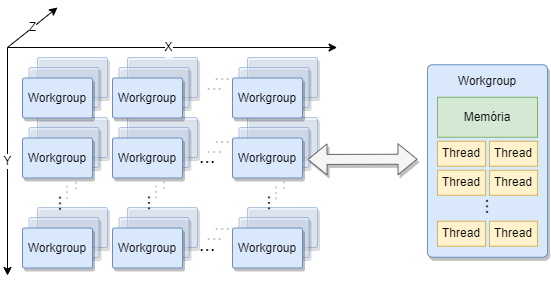
\includegraphics[width=0.75\textwidth]{imagens/WorkgroupsVisualisation2.drawio.png}
  \caption{Distribuição de workgroups e threads em Compute Shaders}
  \label{fig:LABEL_FIG_WORKGROUPS}
\end{figure}

\subsection{O problema da renderização indireta}\label{sec:LABEL_RENDERIZACAO_INDIRETA}

Ao finalizar a execução de um compute shader, as informações processadas podem ser resgatadas da memória de vídeo para a memória principal para serem tratadas pela CPU através dos SSBO. Caso haja a necessidade de utilizar essas informações durante o pipeline de renderização, esses dados necessitam ser repassados novamente à memória de vídeo utilizando \textit{uniforms} de entrada para a execução de um outro programa que contenha ao menos vertex e fragment shaders. Essa renderização indireta pode ser computacionalmente custosa por conta do overhead de transmissão dos dados entre as memórias de vídeo e principal.

\section{Mesh Shaders}\label{sec:LABEL_CHP_1_SEC_D}

Em poucas palavras, mesh shaders são compute shaders capazes de enviar geometrias primitivas diretamente para o rasterizador. Sendo possível realizar todas as funcionalidades que são implementadas do pipeline VTGS, como \textit{occlusion culling}, tesselação e \textit{instancing}, o pipeline que utiliza Mesh shaders é capaz de substituir por completo o pipeline de renderização atual, com a vantagem de ser mais simples e maleável.

Seu principal objetivo é simplificar a esteira de renderização ao remover a etapa de input assembler e integrar as funcionalidades de tesselation evaluation e geometry shaders às etapas iniciais do fluxo. Além disso, mesh shaders visam resolver o problema do gargalo da linearidade dos vertex e index buffers ao permitir que múltiplas subseções de uma malha sejam processadas em paralelo utilizando o conceito de \textit{meshlets}, permitindo assim que geometrias complexas sejam renderizadas de forma mais eficiente. ilustrado na Figura \ref{fig:LABEL_FIG_MESHLETS}.

\begin{figure}
  \centering
  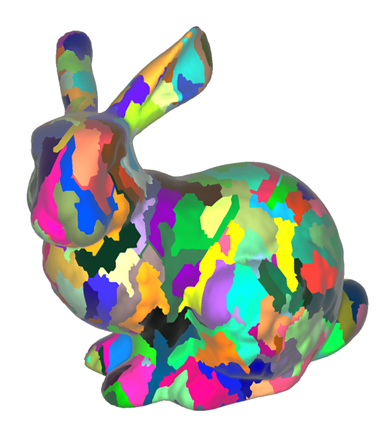
\includegraphics[width=0.25\textwidth]{imagens/MeshletsBunnyNVidia.png}
  \caption{Representação visual de uma geometria subdividida em \textit{meshlets}}
  \label{fig:LABEL_FIG_MESHLETS}
\end{figure}

Mesh shaders permitem que os desenvolvedores gerenciem melhor o uso dos recursos utilizados pelas GPUs. Diferentemente da esteira vigente, esta nova abordagem possibilita que um dado lido pela memória principal permaneça na memória de video até quando for necessário.

Dado seu modelo de computação similar aos compute shaders, mesh shaders facilitam a geração de malha procedural diretamente pela GPU. Processo este que era inflexível, limitado e não performático ao se utilizar TCS, TES e geometry shaders no pipeline VTGS.

Como restrição, Mesh shaders necessitam da alocação prévia de recursos em tempo de compilação. Durante a escrita código do shader, deve-se definir a quantidade de threads, o tipo de primitivo de saída e, por fim, o número máximo de primitivos e vértices gerados por workgroup. Além disso, a primeira geração de hardwares que suportam mesh shaders contém restritas limitações no número máximo de primitivos gerados por workgroup. Por conta disso, para evitar a alocação desnecessária de recursos, é desejável que se tenha um balanceamento entre estes parâmetros.

\subsection{Task Shaders}\label{sec:LAVEL_CHP_1_SEC_TASK_SHADERS}

O pipeline baseado em mesh shaders inclui uma extensão programável chamada de \textit{task shaders} (ou \textit{amplification shader}, em DirectX). Assim como ilustrado na Figura \ref{fig:LABEL_FIG_FLUXO_TASK_MESH_SHADERS}, task shaders são etapas que opcionais antecedem a execução de mesh shaders e tem como principal objetivo a gestão dinâmica de sua carga de trabalho. Task shaders, assim como mesh shaders, também possuem dados de entrada e saída definidas pelo usuário e trabalham com o conceito de workgroups como vistos em compute shaders.

Cada workgroup de um task shader pode ou não emitir uma instancia de mesh shader. Um exemplo de caso de uso é a implementação do \textit{occlusion culling} durante as etapas iniciais do pipeline. O occlusion culling é o processo que se refere à omissão de malha que não será exibida na imagem final, evitando eventuais desperdícios de processamento e no uso de recursos da GPU.

\begin{figure}
  \centering
  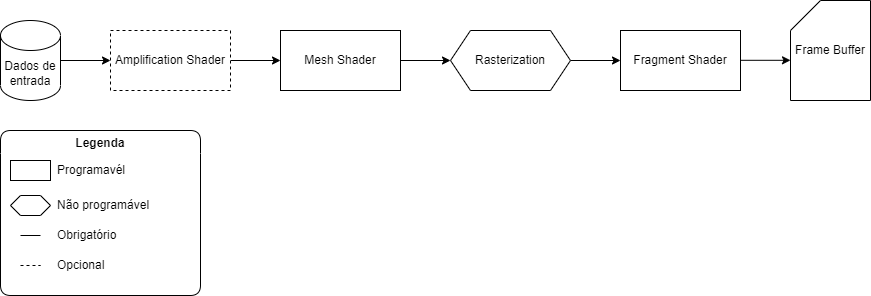
\includegraphics[width=1\textwidth]{imagens/PipelineRenderizacaoOpenGL-Mesh_Shader.png}
  \caption{Pipeline Utilizando Mesh Shaders}
  \label{fig:LABEL_FIG_FLUXO_TASK_MESH_SHADERS}
\end{figure}

%%\codec{Definições iniciais mesh shader}{alg:LABEL_CODE_1}{codigos/codigo-c.txt}


%%\textcolor{red}{TODO: Melhorar sessão de limitações}


%%\textcolor{red}{TODO: Organizar e melhorar figuras}
\chapter{Experimentos e Resultados}\label{chp:LABEL_EXPERIMENTOS}

Neste capítulo abordaremos a aplicação construída para este trabalho com o objetivo de comparar a execução do algoritmo do caso de estudo em duas diferentes implementações: renderização indireta através de compute shaders e renderização direta via mesh shaders.

\section{Ferramenta desenvolvida}\label{sec:LABEL_FERRAMENTA_DESENVOLVIDA}

Visando maior controle sob a esteira de renderização, foi proposto para este trabalho uma aplicação escrita em código aberto utilizando a API gráfica OpenGL e a biblioteca multimídia \textit{SDL2} capaz de compilar e executar compute e mesh shaders. A ferramenta permite também a analise de desempenho ao exibir estatísticas relevantes sobre o uso dos recursos gráficos do computador. A figura \ref{fig:LABEL_FIG_MESH_SHADER_TOOL} apresenta a tela inicial do programa e suas configurações. O código fonte da aplicação pode ser encontrado no repositório público do \textit{GitHub}.\footnote{https://github.com/Vinicius-Asse/marching-cubes}

\begin{figure}
\centering
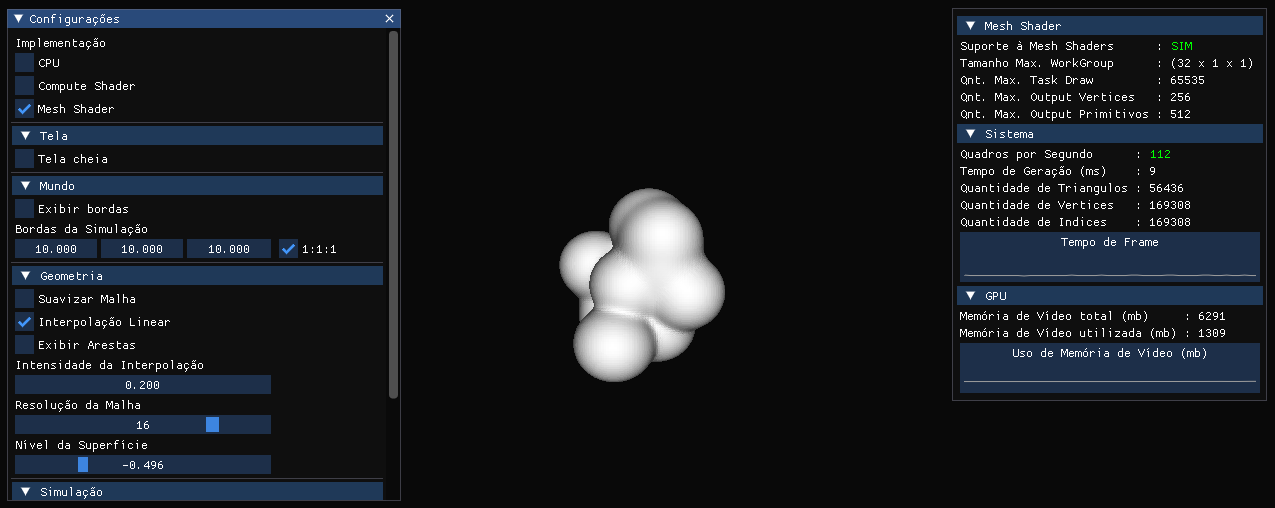
\includegraphics[width=1\textwidth]{imagens/InterfaceFerramenta.png}
\caption{Tela inicial da ferramenta desenvolvida para este estudo}
\label{fig:LABEL_FIG_MESH_SHADER_TOOL}
\end{figure}

\subsection{Funcionalidades}\label{sec:LABEL_FERRAMENTA_DESENVOLVIDA_FUNCIONALIDADES}
Nossa ferramenta é capaz observar se o computador que a executa possui suporte aos mesh shaders e de monitorar a utilização de recursos em tempo de execução. A figura \ref{fig:LABEL_FIG_FUNC_FERRAMENTA} ilustra a interface exibida durante a execução do programa. A tabela \ref{TBL:DESCRICAO_INFO_FERRAMENTA} descreve essas informações.

\begin{figure}
\centering
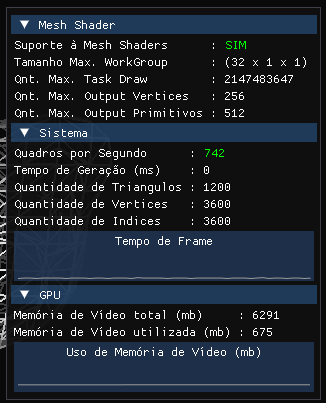
\includegraphics[width=0.5\textwidth]{imagens/FuncionalidadesFerramenta.png}
\caption{Tela inicial da ferramenta desenvolvida para este estudo}
\label{fig:LABEL_FIG_FUNC_FERRAMENTA}
\end{figure}

\begin{center}
\begin{table}
\begin{tabular}{|m{10em} | m{4em} | m{19em} |} 
 \hline
 Campo & Tipo & Descrição  \\
 \hline
Suporte à Mesh Shaders & Boolean & Verdadeiro se e somente se existe suporte ao OpenGL 4.6 e à extensão \textit{GL\_NV\_mesh\_shader} \\ \hline
Tamanho Max. WorkGroup & String & Quantidade máxima de Workgroups despachados por instância de Task/Mesh Shaders  \\ \hline
Qnt. Max. Task Draw & Integer & Quantidade máxima de instâncias de Mesh shaders instanciados por Task Shader   \\  \hline
Qnt. Max. Output Vértices & Integer & Quantidade máxima de vértices gerados por Workgroup \\  \hline
Qnt. Max. Output Primitives & Integer & Quantidade máxima de primitivos gerados por Workgroup \\  \hline
Quadros por Segundo & Integer & Quantidade de quadros (frames) renderizadas por segundo \\  \hline
Tempo de Geração (ms) & Integer & Tempo de geração da malha utilizando o algoritmo de Marching Cubes em milissegundos \\  \hline
Quantidade de Triângulos & Integer & Quantidade total de triângulos renderizados \\  \hline
Quantidade de Vértices & Integer & Quantidade total de vértices renderizados \\  \hline
Quantidade de Indices & Integer & Quantidade total de indices renderizados \\  \hline
Memória de video total (mb) & Integer & Capacidade total de memória de vídeo em mega bites \\  \hline
Memória de video utilizada (mb) & Integer & Quantidade de memória de vídeo utilizada em mega bites \\  \hline

\end{tabular}
\caption{Informações monitoradas durante a execução do programa}
\label{TBL:DESCRICAO_INFO_FERRAMENTA}
\end{table}
\end{center}

\section{Metodologia dos experimentos}\label{sec:LABEL_AMBIENTE_EXPERIMENTOS}

Visto que o objetivo do trabalho é estudar o comportamento do pipeline de renderização em contexto de aplicações em tempo real, os dados observados foram relacionados ao tempo de geração de frame para cada uma das seguintes implementações:

\begin{itemize}
    \item Em memória via CPU: a iteração sobre os pontos são feitas linearmente em memória principal diretamente pela CPU. O resultado do processo são os index e vertex buffers que são repassados para a esteira VGTs para renderização;
    \item Renderização indireta via compute shaders: os pontos são distribuídos entre as threads dos workgroups. Cada thread pode realizar seu processamento de forma completamente paralela das demais. O resultado do processo são os index e vertex buffers que são renderizados de forma indireta, conforme abordamos durante a Sessão \ref{sec:LABEL_FLUXO_DOS_DADOS}.;
    \item Renderização direta via mesh shaders: os pontos são distribuídos entre as threads dos workgroups. Cada thread pode realizar seu processamento de forma completamente paralela das demais. O resultado do processo são os index e vertex buffers repassados diretamente para a rasterização e renderização;
\end{itemize}

Todos os testes foram executados em um \textit{desktop} com processador Intel Core i5 10400f, 16 \textit{gibabytes} de RAM, placa de vídeo NVIDIA GeForce GTX 1660 Super e sistema operacional \textit{Windows 11}. 

\section{Resultados}\label{sec:LABEL_RESULTADOS}

\begin{figure}
\centering
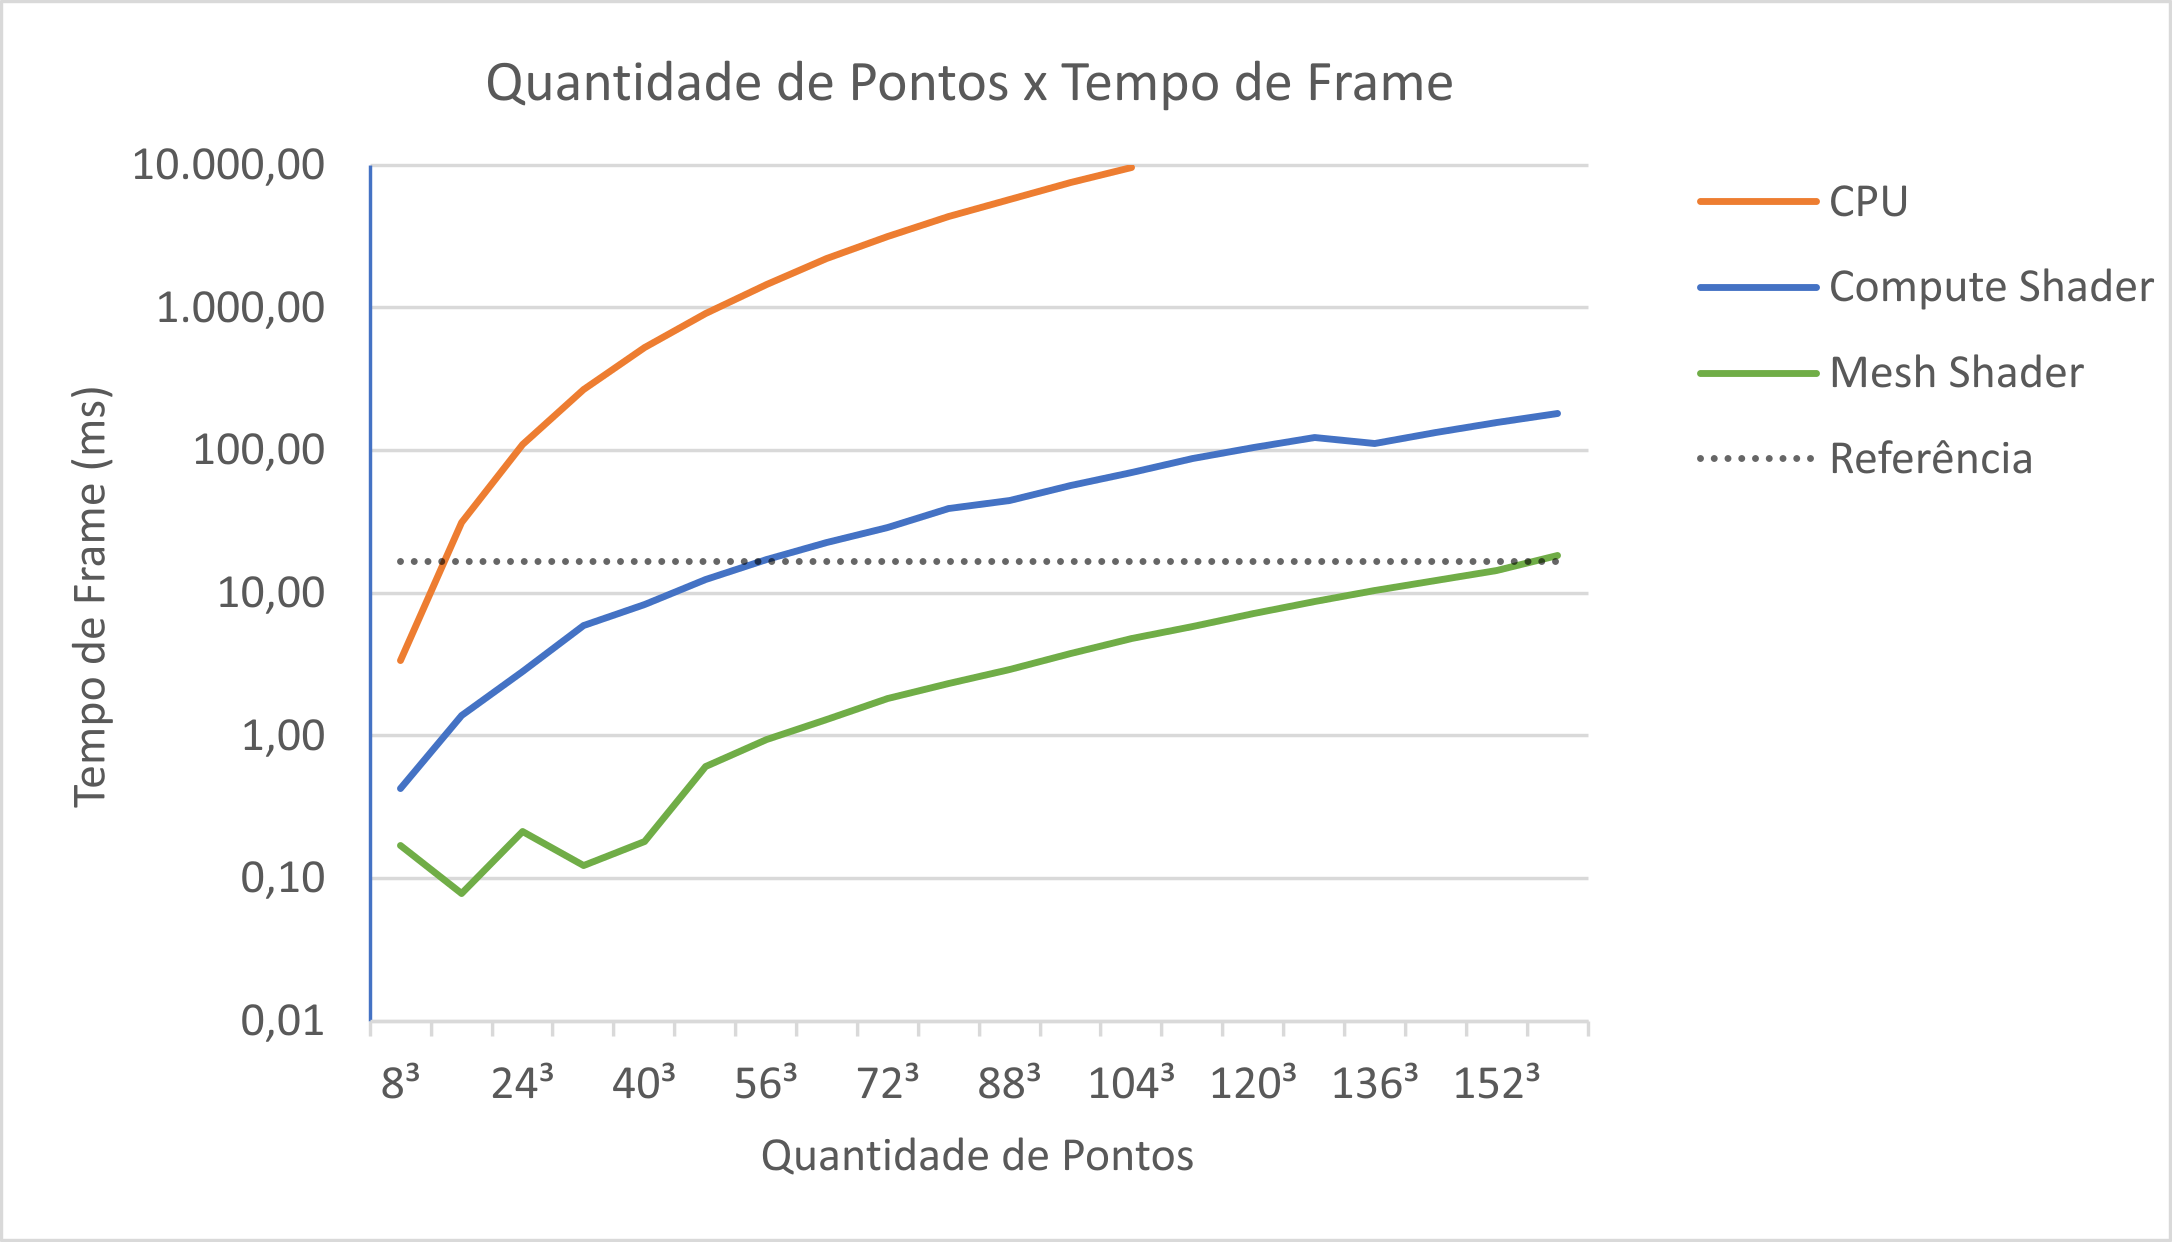
\includegraphics[width=1\textwidth]{imagens/PontosXTempoFrame.png}
\caption{Relação entre a quantidade de pontos e tempo de frame}
\label{fig:LABEL_FIG_PONTOS_X_TEMPO}
\end{figure}

Durante a execução do algoritmo utilizando em mesh shaders, conseguimos observar uma significativa redução no tempo de geração de frames em relação as demais implementações, se mantendo abaixo do limiar desejável de ~16,666 ms de tempo de frame até que a quantidade de pontos atingisse um total de $152^3$ pontos. A figura \ref{fig:LABEL_FIG_PONTOS_X_TEMPO} ilustra a diferença entre o tempo de geração de imagens entre as implementações. A visualização dos ganhos do uso de Mesh shaders em comparação aos compute shaders é detalhado pela Tabela \ref{TBL:TEMPO_FRAME_IMPL}. 

\begin{center}
\begin{table}
\begin{tabular}{|c | c | c | c |} 
 \hline
 Qnt. de Pontos & Compute Shaders (ms) & Mesh shaders (ms) & SpeedUp  \\
 \hline\hline
8³ & 0,424046 & 0,169582 & 2,5 \\ \hline
16³ & 1,377016 & 0,078685 & 17,5 \\ \hline
24³ & 2,808765 & 0,213918 & 13,1 \\ \hline
32³ & 5,886228 & 0,122899 & 47,9 \\ \hline
40³ & 8,252874 & 0,180791 & 45,6 \\ \hline
48³ & 12,484848 & 0,612670 & 20,4 \\ \hline
56³ & 17,285714 & 0,940276 & 18,4 \\ \hline
64³ & 22,793103 & 1,294455 & 17,6 \\ \hline
72³ & 28,800000 & 1,821869 & 15,8 \\ \hline
80³ & 39,000000 & 2,329283 & 16,7 \\ \hline
88³ & 44,647059 & 2,915858 & 15,3 \\ \hline
96³ & 56,357143 & 3,769663 & 15,0 \\ \hline
104³ & 70,250000 & 4,819277 & 14,6 \\ \hline
112³ & 87,375000 & 5,834586 & 15,0 \\ \hline
120³ & 105,222222 & 7,161017 & 14,7 \\ \hline
128³ & 122,857143 & 8,684211 & 14,1 \\ \hline
136³ & 111,125000 & 10,376238 & 10,7 \\ \hline
144³ & 133,000000 & 12,162162 & 10,9 \\ \hline
152³ & 156,250000 & 14,400000 & 10,9 \\ \hline
160³ & 181,073171 & 18,281250 & 9,9 \\ [1ex] \hline
\end{tabular}
\caption{Tempo de geração de frame durante a execução de marching cubes}
\label{TBL:TEMPO_FRAME_IMPL}
\end{table}
\end{center}

Em ambas as implementações não foi notado grandes variações quanto a quantidade de memória dedicada de vídeo foi alocada. Entretanto, a implementação em mesh shaders mostrou um uso mais estável do uso dos recursos. Conforme ilustrado na Figura \ref{fig:LABEL_USO3D_GPU}, onde o intervalo 1 representa a implementação em compute shaders e o intervalo 2 mesh shaders, a maior diferença observada foi em questão do uso dos mecanismo 3D da GPU, que chegou a $92\%$ em testes mais pesados em contraste da média de uso de aproximadamente $20\%$ vista em compute shaders.

Acreditamos que tais resultados sejam consequência da renderização indireta necessária em compute shaders. Parte do processamento é delegado da GPU para a CPU. Em cargas mais altas, a GPU se encontrava osciosa enquanto a CPU resgatava e repassava os SSBOs em forma de vertex e index buffers para alimentar a esteira VGTs.


\begin{figure}
\centering
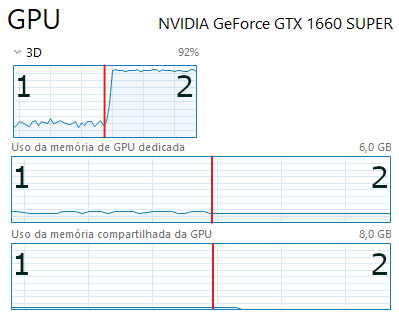
\includegraphics[width=0.75\textwidth]{imagens/Uso3DGPU.png}
\caption{Uso dos recursos da GPU durante a execução do algoritmo.}
\label{fig:LABEL_USO3D_GPU}
\end{figure}

\chapter{Conclusão}\label{chp:LABEL_CONCLUSAO}

Neste capítulo concluiremos o trabalho e fornecemos sugestões de possíveis continuações do estudo para o futuro.

\section{Conclusão}\label{sec:LABEL_CONCLUSAO_SEC_A}

Embora o conceito de mesh shaders seja um avanço disruptivo para a computação gráfica, seu uso por si só não garante ganhos de performance quando comparado ao pipeline atual. Fica em cargo dos desenvolvedores utilizar suas funcionalidades eficientemente afim de aprimorar seu desempenho.

Trazendo para o contexto de geração de malha procedural, mesh shaders aprimoram o fluxo de dados permitindo que grandes lotes de geometria sejam processadas e renderizadas de forma eficiente sem a necessidade de copiar os dados na memória principal. Embora haja a necessidade da alocação previa dos recursos, não observamos um uso significativo de memória dedicada de video durante a implementação de marching cubes em mesh shaders. A flexibilidade em seus atributos de entrada permitem que diversos algoritmos sejam implementados utilizando de forma ideal os recursos disponíveis pelos componentes de aceleração gráfica.

\section{Trabalhos Futuros}\label{sec:LABEL_CONCLUSAO_SEC_B}

Visando explorar todas os recursos providos por mesh shaders, propomos os seguintes trabalhos futuros:

\begin{itemize}
    \item Implementação de nível de detalhe dinamicos;
    \item Utilização de task shaders para aplicar técnicas de \textit{culling} e \textit{instancing};
    \item Virtualização de geometria com mesh shaders;
\end{itemize}
\pagebreak

%%%%%%%%%%%%%%%%%%%%%%%%%%%%%%%%%%%%%%%%%%%%%%%%%%%%%%%%%%%%
% B I B L I O G R A F I A
%%%%%%%%%%%%%%%%%%%%%%%%%%%%%%%%%%%%%%%%%%%%%%%%%%%%%%%%%%%%
% Retirar esta parte se o trabalho não tiver bibliografia
\makebibspage{elementos-postextuais/referencias}

%%%%%%%%%%%%%%%%%%%%%%%%%%%%%%%%%%%%%%%%%%%%%%%%%%%%%%%%%%%%
% A P E N D I C E
%%%%%%%%%%%%%%%%%%%%%%%%%%%%%%%%%%%%%%%%%%%%%%%%%%%%%%%%%%%%
% Retirar esta parte se o trabalho não tiver anexos
%\appendix
%\input{elementos-postextuais/apendice}

\end{document}
